\section{Zielsetzung}

Laser stellen für die Physik ein sehr wichtiges Instrument dar. Durch ihren Ausstoß von kohärentem Licht in einem sehr kleinen Frequenzspektrum eignen sie
sich ideal, um zum Beispiel atomare Strukturen zu untersuchen. In diesem Versuch soll konkret die Funktionsweise eines Diodenlasers erprobt werden. Hierfür wird dieser
verwendet, um Rubidium zu untersuchen und seine Fluoreszenz nachzuweisen.


\section{Theorie}
\label{sec:Theorie}

Es bedarf dafür zunächst einer Erläuterung der physikalischen Grundlagen, die zum Verständnis der Funktionsweise des Diodenlasers notwendig sind. Es handelt sich
hierbei um das Konzept der Photonenemission sowie der Funktionsweise von Halbleitern und Dioden.


\subsection{Absorption und Emission von Photonen}
\label{subsec:absorption}

Ein quantenmechanisches System kann nicht beliebige Energien annehmen. Es liegen lediglich verschiedene diskrete Energieniveaus vor, zwischen denen Übergänge
stattfinden können. Ein Beispiel hierfür wäre ein Atom, welches ein Photon absorbiert und dadurch in einen angeregten Zustand mit höherer Energie wechselt.
Voraussetzung hierfür ist, dass die Energie des Photons exakt der Differenz beider Energieniveaus entspricht.
\newline
Befindet sich das Atom im angeregten Zustand, gibt es nun zwei Möglichkeiten, wie es in seinen Grundzustand zurückkehren kann. Zum einen ist eine spontane
Emission eines Photons möglich. Diese wird lediglich durch Quantenfluktuationen ausgelöst und ist nicht vorherzusagen. Die Energie des hierbei emittierten
Photons entspricht exakt der Energiedifferenz von angeregtem Zustand und Grundzustand. Seine Ausbreitungsrichtung, Polarisation und Phase sind hierbei beliebig.
\newline
Wechselwirkt das angeregte Atom jedoch mit einem Photon der richtigen Energie, kann es auch zu stimulierten Emissionen kommen. Die hierfür notwendige Energie 
des einfallenden Photons ist erneut die Differenz der beiden Energieniveaus. Auch hierbei wird ein Photon identischer Energie emittiert, das sich aber im
Gegensatz zur spontanen Emission immer in Richtung des einfallenden Photons bewegt und sich auch in Phase und Polarisation nicht von diesem unterscheidet.
\newline
Es kann also durch stimulierte Emission die Anzahl an Photonen einer bestimmten Wellenlänge stark verstärkt werden. Genau dieser Prozess wird sich im aktiven
Medium eines Lasers zu Nutzen gemacht. Damit die stimulierte Emission im Gegensatz zur spontanen Emission dominiert, muss ein Zustand erreicht werden, bei dem
der energetisch höherer Zustand häufiger besetzt ist als der Grundzustand. Ein solcher Zustand wird auch Besetzungsinversion genannt.
\newline
Um eine Besetzungsinversion zu erreichen, sind jedoch mehr als zwei Zustände nötig. Dies liegt daran, dass die Übergangswahrscheinlichkeit zwischen zwei Zuständen
gleich ist, unabhängig davon, von welchem Zustand ausgegangen wird. Dies hat zur Folge, dass in einem Zwei-Niveau-System keine Besetzungsinversion, sondern höchstens
eine gleichmäßige Besetzung beider Zustände, erreichbar ist. Das einfachste System, für das dies hingegen möglich ist, ist demnach ein Drei-Niveau-System. Eine
schematische Darstellung eines solchen ist in \autoref{fig:dreiniveau} zu sehen.

\begin{figure}[H]
    \centering
    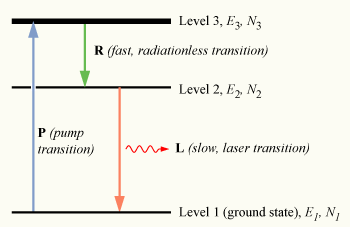
\includegraphics[width=\textwidth]{data/dreiniveau.png}
    \caption{Schematische Darstellung eines Drei-Niveau-Systems \cite{Dreiniveau}.}
    \label{fig:dreiniveau}
\end{figure}
\noindent
In einem System wie diesem ist es möglich, dass ein Großteil der Teilchen sich außerhalb des Grundzustands befindet, insofern das mittlere Energieniveau langlebiger
ist als das höchste. Falls dies der Fall ist, werden sich die Teilchen langfristig im mittleren Niveau ansammeln, da mehr Teilchen aus dem hohen in den mittleren Zustand
übergehen als solche, die vom mittleren in den Grundzustand übergehen. 


\subsection{Dotierung und Dioden}

Von einem dotierten Halbleiter ist die Rede, wenn in einen Halbleiter Fremdatome eingebracht werden, um seine Leitfähigkeit zu beeinflussen. Es wird prinzipiell
zwischen n-dotierten und p-dotierten Halbleiter unterschieden. Relevant dafür ist die Anzahl an Valenzelektronen der Elemente des Halbleiters und der Fremdatome.
Werden Fremdatome in einen Halbleiter hinzugefügt, die ein Valenzelektron mehr haben als die Atome des Halbleiters, wird dies als n-Dotierung bezeichnet,
da durch das Hinzufügen ein freies Elektron, also eine freie negative Ladung entsteht. Bei der p-Dotierung hingegen wird ein Fremdatom mit einem Valenzelektron weniger hinzugefügt,
wodurch ein sogenanntes Elektronenloch im Halbleiter entsteht. Dieses Loch wiederum ist auch frei beweglich und verhält sich wie eine freie positive Ladung.
\newline
Werden nun ein p-dotierter Halbleiter und ein n-dotierter Halbleiter in Kontakt gebracht, so ist die Rede von einem pn-Übergang. Ein solcher pn-Übergang bildet den Kern einer Diode.
An der Fläche, an der sich die verschieden dotierten Halbleiter berühren, können sich die Elektronen zwischen den Halbleitern frei bewegen. Dies hat zur Folge, dass
im n-dotierten Teil eine positiv geladene Zone und im p-dotierten Teil eine negativ geladene Zone entsteht. Aufgrund der Coulomb-Abstoßung werden dann neu entstehende freie Ladungen
aus dem pn-Übergang gesaugt, weshalb der pn-Übergang als Isolator fungiert und auch als Sperrschicht bezeichnet wird.
\newline
Durch Anlegen einer Spannung an die Diode können, abhängig von der Polung, zwei Dinge passieren. Wird die n-dotierte Seite mit dem negativen Pol verbunden, führt dies in der Diode
zu einem elektrischen Feld, das dem Feld in der Sperrschicht entgegengesetzt ist. Ab einer gewissen Spannung gleichen sich diese Felder genau aus und für noch höhere Spannungen kann
dann Strom durch die Diode fließen. Eine Diode, an der eine so gepolte Spannung anliegt, ist in \autoref{fig:diode} zu sehen.

\begin{figure}[H]
    \centering
    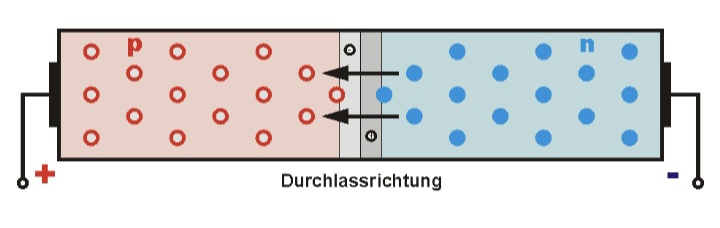
\includegraphics[width=\textwidth]{data/diode.jpg}
    \caption{Schematische Darstellung einer Diode in Durchlassrichtung \cite{Diode}.}
    \label{fig:diode}
\end{figure}
\noindent
Eine gegensätzlich gepolte Spannung hingegen würde das in der Diode vorhandene Feld nur verstärken. In dieser Richtung ist also auch für höhere Spannungen kein Stromfluss möglich.
\newline
Wird die Diode in Durchlassrichtung gepolt, führt dies dazu, dass Elektronen durch den p-dotierten Halbleiter fließen und dort mit den Elektronlöchern rekombinieren. Durch diesen
Prozess werden Photonen emittiert. Bei einer ausreichend hohen Spannung kann dies zu einer Besetzungsinversion führen. Dadurch wird stimulierte Emission in der Diode möglich
und es kann kohärentes Licht hoher Intensität entstehen.


\subsection{Aufbau des Diodenlasers}

Das wichtigste Bauteil des Diodenlasers ist sein Chip. Eine schematische Darstellung der Seitenansicht eines solchen ist in \autoref{fig:diodechip} zu sehen.

\begin{figure}[H]
    \centering
    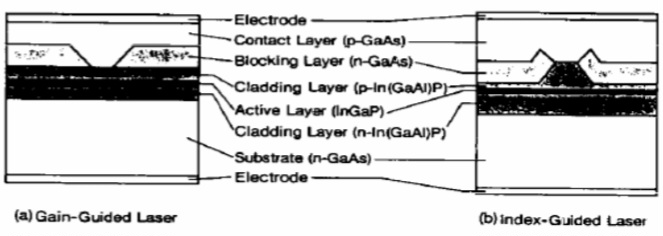
\includegraphics[width=\textwidth]{data/chip.jpg}
    \caption{Seitenansicht eines Dioden Chips \cite{Anleitung60}.}
    \label{fig:diodechip}
\end{figure}
\noindent
Den Kern des Chips bildet der pn-Übergang, der für Diodenlaser als aktives Medium (Active Layer) fungiert. Umgeben ist dieser von p-dotierten und n-dotierten Schichten
(Cladding Layers). Der Querschnitt wird zu einer Seite hin von einem undurchlässigen Reflektor begrenzt. Zur anderen Seite hin ist die Begrenzung halbdurchlässig, um
einen Teil des Lasers auszukoppeln und nutzbar zu machen. Da sich zwischen den beiden Begrenzungen stehende Wellen bilden, wird dieser Teil des Chips auch interner
Resonator genannt. Es kann so hier zu stimulierten Emissionen kommen und der Laser sich so stetig verstärken.
\newline
Der Teil des Laserstrahls, der aus dem Chip ausgekoppelt wird, durchläuft anschließend den sogenannten Littrow-Aufbau. Die Skizze eines solchen ist in
\autoref{fig:littrow} zu sehen.

\begin{figure}[H]
    \centering
    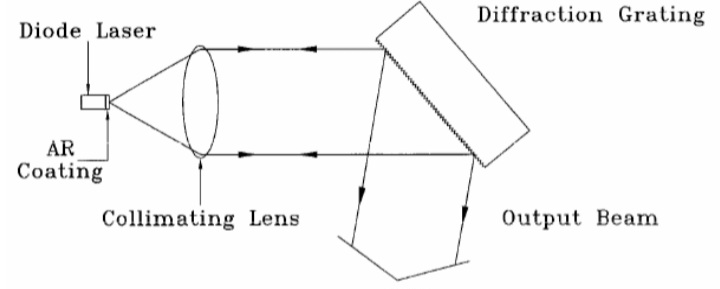
\includegraphics[width=\textwidth]{data/littrow.jpg}
    \caption{Skizze eines Littrow-Aufbaus \cite{Anleitung60}.}
    \label{fig:littrow}
\end{figure}
\noindent
Der ausgetretene Strahl durchläuft zunächst eine Kollimator-Linse. Diese transformiert den Strahl zu einer planare Wellenfront. Die Wellenfront trifft dann auf
ein Beugungsgitter, welches in einem präzisen Winkel angeordnet ist, um exakt die erste Beugungsordnung zurück in den Laser zu reflektieren. Es bildet sich so
zwischen Gitter und hinterer, undurchlässiger Begrenzung des Chips eine weitere stehende Welle, weshalb dieser Teil auch als externer Resonator bezeichnet wird.
Die nullte Ordnung, oder direkte Reflexion, ist dann der final ausgegebene Laser.


\subsection{Absorptionsspektrum von Rubidium}

Durchläuft ein Laserstrahl ein Rubidiummedium werden ein Teil seiner Photonen von diesem absorbiert. Die Energieniveaus in Rubidium sind zusammen mit dem erwarteten Absorptionsspektrum
von Rubidium in \autoref{fig:niv} dargestellt.

\begin{figure}[H]
    \centering
    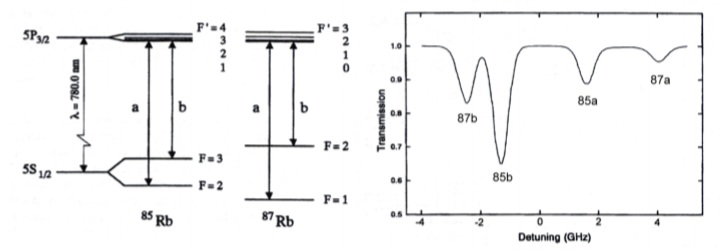
\includegraphics[width=\textwidth]{data/niveaus.jpg}
    \caption{Aufbau des Versuches \cite{Anleitung60}.}
    \label{fig:niv}
\end{figure}
\noindent
Hierbei können, wie bereits in \autoref{subsec:absorption} beschrieben, nur solche Photonen absorbiert werden, deren Energie der Differenz zweier Energieniveaus in Rubidium entspricht.
Dies hat zur Folge, dass nur bei genau diesen Wellenlängen ein Einbruch in der Intensität des Lasers messbar ist.
